\documentclass[a4paper,notitlepage]{article}
\usepackage{ssn-format}
\title{PFS ICS network plan and configuration}
\author{PFS ICS Team}
%\date{2012--08--28}
\begin{document}

\SSNID{00010}
\SSNREV{002}
\SSNCATEGORY{ICS}
\SSNChangeRecord{Rev.001 / First Release / 2015--03 \\
Rev.002 / Updated fiber connections / 2015--10}
\SSNReference{(none)}
\SSNAttachment{(none)}
\SSNWritten{PFS ICS Team}
%\drafttrue

\ssnhead

\section{Abstract}

This note contains infrastructural design on PFS ICS network, from hardware 
design (L1, or so-called L0) to transport layer (L4), but not including L5 
to L7. 
Also, this note covers management items and configurations for network 
infrastructure, such as monitoring of network hardware, address distribution, 
network management, and real configurations on (cisco) switches and computers. 

\section{Applicable documents}

Following ICDs and requirements are covered and/or referenced in this note. 

\begin{description}
  \item[ICD 70] PFS Fibers from CB2F patch panel to subsystems
\end{description}


\section{Requirements to PFS ICS network}

Requirements to PFS ICS network are imposed from both technical aspect and 
management aspect (mostly from Subaru). 

Requirements on management aspect are:

\begin{itemize}
  \item Subaru standard recommendation of network switches are Cisco 
    2960X-24TD-L or 2960CG-8TC-L to keep variety of network switches used 
    at the summit as minimum as possible both to keep switch management simple 
    and to keep number of spare parts to be small. If not possible, Cisco 
    2960X, 2960CG, or 3650 are possible.
  \item Network switch shall be managed and monitored from Subaru CDM, and 
    follow standard configuration (e.g. VLAN, remote access) of CDM.
  \item All PFS network components shall be on the single subnet (PFS-LAN) and 
    single VLAN ID, which will be assigned from Subaru with fitting Subaru's 
    configuration. Also seemless access from Subaru network (incl Hilo, VPN) 
    to PFS LAN for remote maintenance and operation are required, although 
    security of instrument operation need to be secured in a required level.
    Discussions and negotiations with Subaru are planned on this point. 
  \item All connections to subaru dome from computer roon at the control 
    building 2F (CB2F) are in fiber connection. 
  \item Static IP address assignment is desired.
\end{itemize}

PFS ICS network is in coordination to satisfy and be capable to accept desire 
from technical design of PFS instrument, requirements on technical aspect are 
not solid and will be added or modified by updates and developments of PFS ICS 
hardware. For now, following requirements are pointed: 

\begin{itemize}
  \item Core switches for PFS-LAN are hosted at CB2F, and all distribution 
    switches connect only to core switches but not peer connection to other 
    distribution switches.
  \item Specially required data flow rate from/to distribution switches are: 
    TUE-IR (SpS) is $>$ 2Gbps, storage at CB2F is $>$ 4Gbps.
    1Gbps link is assumed to Subaru E-LAN (TBC).
  \item Required and possible optical fiber connection to distribution switches 
    are: TUE-IR (SpS) is up to 4 SM fiber pairs in 1Gbps or 10Gbps, PF and 
    TUE-Opt is 2 MM fiber pairs in 1Gbps, and Cs is 1 MM or SM fiber pairs in 
    1Gbps. Assigned fibers are listed in ICD-70.
  \item On instrument exchange, fibers to PF/TUE-Opt need to be exchanged and 
    permanent connection for these fibers are not possible, Cs and Cs-Standby 
    fibers will be dedicated to PFS and permanent connection are possible.
\end{itemize}


\section{Network design}

\subsection{L0-2: Physical layer, wiring design, and datalink}

For physical layer, we take simple configuration without selectable definitions 
on components as followings:

\begin{itemize}
  \item All fiber networks are by 1000BASE-LX with SM or MM fiber pair. We may 
    need MCP for MM connections over 300m length (most of connections between 
    core and distribution), but to insert or not depends on hardware capacity 
    to put MCP fiber.
  \item PFS LAN will not share one switch by more than two VLANs, except for 
    management VLAN operated by Subaru CDM. Connection(s) between core switch 
    on PFS-LAN and Subaru, as well as PFS core and some distribution switches 
    (Cs and SpS) are by tag-VLAN (trunk port). 
  \item No switch management or monitoring network (VLAN) by PFS ICS operation. 
    Monitoring by SNMP or management by telnet used for PFS ICS operation are 
    done within PFS-LAN. Also no STP will be used for PFS ICS operation.
\end{itemize}

From these design concepts, physical layer and wiring are designed as following 
connections, physical wiring diagram to distribution layer are shown in 
Figure.~\ref{fig:network_physical}. 
Two connections of PCIe bus extender are purely peer-to-peer connection between 
its host and target devices, and no connection to PFS-LAN. 

\begin{description}
  \item [CB2F -- SpS] 4x 1Gbps SM 1000BASE-LX link in LACP.
  \item [CB2F iSCSI storage] 8x 1Gbps metal link in iSCSI logical layer 
    multipath device mapping, no configuration is required on switch. 
    Also 2 storage management network (1Gbps metal) is connected.
  \item [CB2F -- PF or TUE-Opt standby] 2x 1Gbps MM/62.5 1000BASE-LX link 
    to two points (PFI and cal-lamp) and 2x SM PCIe optical link are used. 
    Switch all fibers at both end during instrument exchange works.
  \item [CB2F -- Cs or Cs standby] 1x 1Gbps SM 1000BASE-LX link. Fibers and 
    their connections are permanent, and connection will be switched at Cs 
    frange by its auto-connector on Cs instrument exchange.
  \item [CB2F -- E-LAN] PFS-LAN and E-LAN will be (fully) routed at Subaru 
    network switch, core switch just provide (some) 1Gbps metal connection(s).
\end{description}

\begin{figure}[htb]
  \begin{center}
    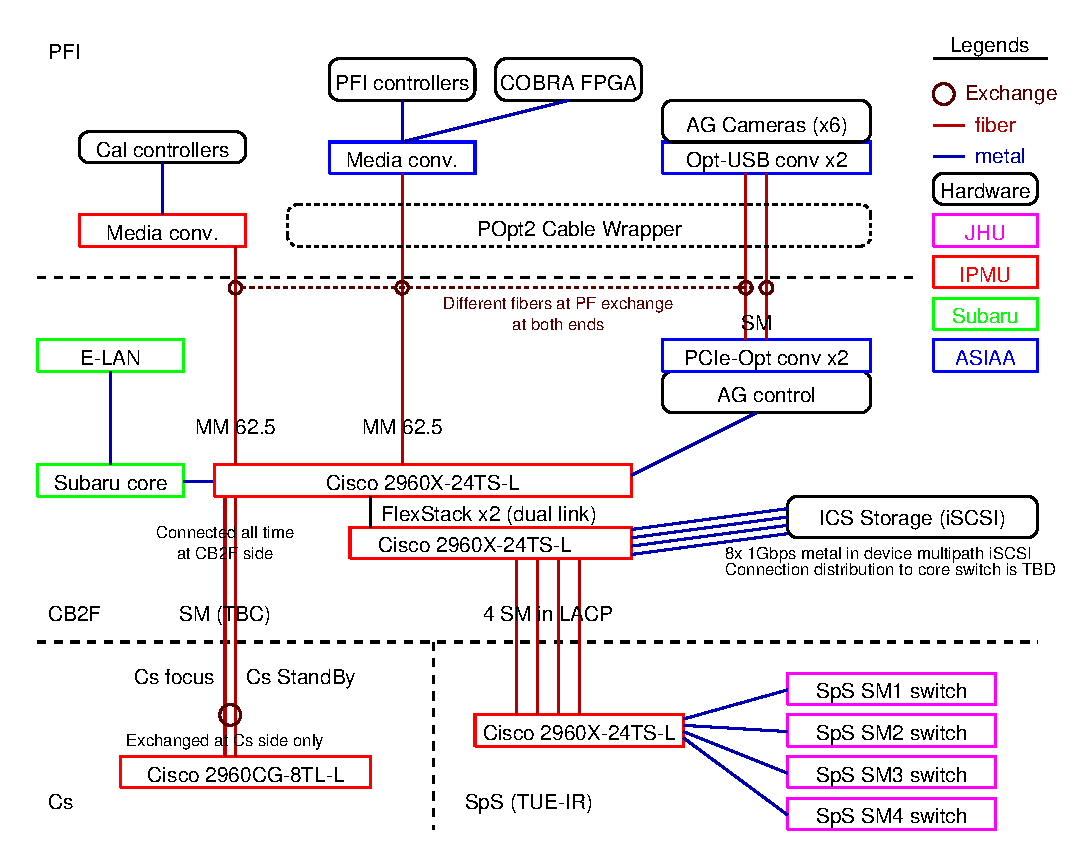
\includegraphics{pfs_network_physical.eps}
  \end{center}
  \caption{PFS ICS network physical wiring diagram}
  \label{fig:network_physical}
\end{figure}


\subsection{L3, Network layer design}

\subsubsection{IP address management}

PFS LAN has assigned IP address range of 133.40.164/23 from Subaru. 
IP address assignment could be divided into subnet to module groups, but 
not yet defined. IP address is to be fixed to function like BCU1-BEE, but not 
fixed to device (MAC address). 

PFS LAN uses DHCP service (dnsmasq) for IP address and hostname management, 
which is configured to assign static lease addresses for operational devices 
and DHCP addresses for temporary use devices such as notebook computers for 
engineering purpose. Devices can get its IP address and hostname from PFS DHCP 
server, but assignment is static as configured in the DHCP server. Also 
dnsmasq provides configurations via DHCP such as hostname defined in static 
lease table, and a DNS service. 

When we exchange device for maintenance or replacement, following tasks need 
to be performed:

\begin{itemize}
  \item Table of IP address and hostname to MAC address shall be modified, but 
    relation between IP address and hostname shall be kept fixed. 
  \item If device is not configured as DHCP, change IP address configuraion 
    of the device.
  \item For computing hardware (which runs OS; Linux) especially for ENUx and 
    xCUy, hostname shall be taken from DHCP server. Actor name and its 
    configuration will be choosen using hostname. Continuity need to be 
    considered at system monitoring, but change of 'computing hardware' should 
    be fine if monitoring is fixed as "hostname" which is equal to service 
    name. 
\end{itemize}

\subsubsection{External connection}

PFS LAN will have full IP routing from/to Subaru network, connection through 
routing device will be filltered by whitelisted IP address. This filter makes 
whitelisted hosts in Subaru network can connect to whitelisted PFS-LAN hosts, 
not to access PFS devices by accident
\footnote{Details are still to be discussed, basically a trade between ease 
of configuration and management of such filtering and a risk of accident and 
security.}

\subsubsection{Hardware connection}

Some CB2F hosts are configured and used as VM host, and their network interface 
are configured as bridge interface
\footnote{Use of bonding/LACP with multiple ports network card is under 
discussion and (technical) investigation.}, without NAPT nor IP forward 
service. 

At least one CB2F host need to be connected to V-LAN network switch, but VM or 
physical is not defined yet. If this one is running as VM, its physical host(s) 
shall have physical connection to V-LAN network switch configured as bridge and 
a serial connection to MLP1 with mapping from VM to physical port. Considering 
redundancy, more than one VM host are better to be configured in the same way, 
and these hosts shall have access (address assigned) to PFS-LAN, but not for 
other networks such as V-LAN. 



\section{Monitoring and remote management}

\subsection{Switch and network flow monitoring}

SNMP based monitoring is planned for network switches. 
Baseline is to use periodic status archive like mrtg or munin for status 
handling and archive (sample in Figure.~\ref{fig:network_munin}), but it could 
be better to integrate somehow to PFS ICS status system like by pushing from 
monitoring system to MHS for some filtered items, but TBD.
Items to be monitored are:

\begin{itemize}
  \item Network flow per port and stack
  \item Switch operation statistics (CPU usage, temperature)
  \item Port and stack operation statistics (connection status and link speed)
\end{itemize}

Control computers and VM hosts are not assumed to be monitored as this, but 
VM hosts at CB2F might be better to be monitored, especially to monitor VM 
clients' network ports. 
SpS access switches which are delivered from JHU will be monitored in some way 
as others, but we need to find some way
\footnote{Monitorable by SNMP or not is not clear.}.

\begin{figure}[htb]
  \begin{center}
    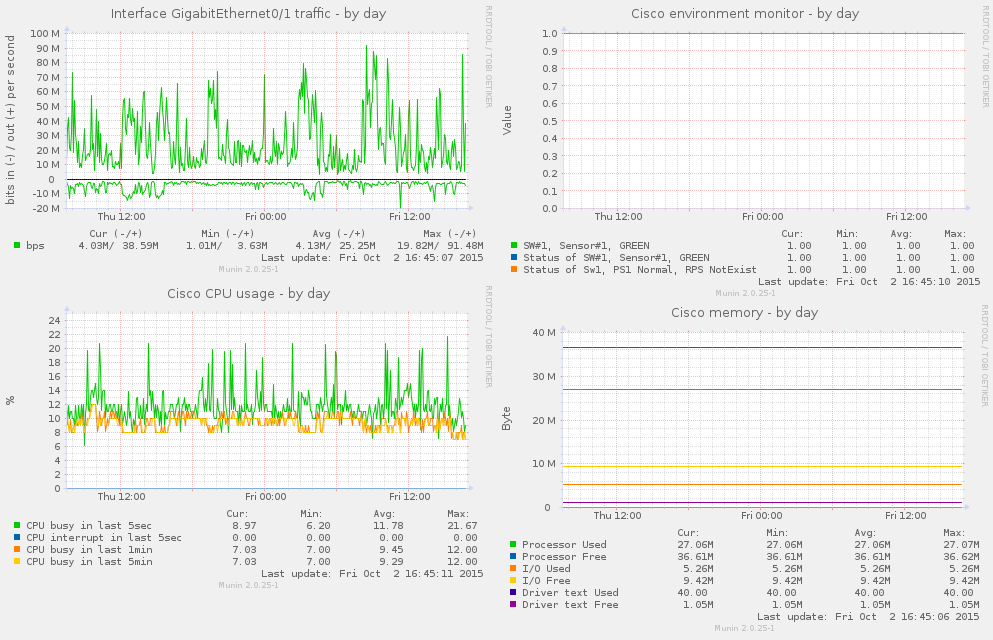
\includegraphics{pfs_network_munin.png}
  \end{center}
  \caption{Sample graphs of monitoring using munin via SNMP}
  \label{fig:network_munin}
\end{figure}

\subsection{Switch remote management}

Network switches are remotely managed normally, configurations are followings: 

\begin{itemize}
  \item No serial or USB console connected for normal operation
  \item Enable telnet connection via management IP address. PFS-LAN network 
    switch will have a IP address of PFS-LAN.
  \item Configuration via SNMP disabled
\end{itemize}

No secured idea has been developed nor defined for SSH or web based access to 
network switches, that SSH or https connection requires complex configurations 
and key management. Since PFS-LAN and management network of Subaru network (by 
CDM) are closed, simple telnet should be fine on security point of view.



\end{document}

